\documentclass{ubicomp2012}
\usepackage{times}
\usepackage{url}
\mdseries\itshape\urlstyle{same}
\usepackage{graphics}
\usepackage{color}
\usepackage{mathtools}
\usepackage{float}
\usepackage[pdftex]{hyperref}
\usepackage{listings}
\lstset{ %
  % language=C,             % the language of the code
  basicstyle=\ttfamily,         % the size of the fonts that are used for the code
  showspaces=false,             % show spaces adding particular underscores
  showstringspaces=false,       % underline spaces within strings
  showtabs=false,              % show tabs within strings adding particular underscores
  tabsize=2,                    % sets default tabsize to 2 spaces
  captionpos=b,                 % sets the caption-position to bottom
  breaklines=true,              % sets automatic line breaking
  breakatwhitespace=false     % sets if automatic breaks should only happen at witespace
}
\hypersetup{%
pdftitle={Thinges for Dummies},
pdfauthor={David Thomas, Egil Hansen},
pdfkeywords={UI-less devices, smart homes, remote control, infrastructure.},
bookmarksnumbered,
pdfstartview={FitH},
colorlinks,
citecolor=black, filecolor=black, linkcolor=black, urlcolor=black,
breaklinks=true, }
\newcommand{\comment}[1]{}
\definecolor{Orange}{rgb}{1,0.5,0}
\newcommand{\todo}[1]{\textsf{\textbf{\textcolor{Orange}{[[#1]]}}}}

\pagenumbering{arabic}  % Arabic page numbers for submission.  Remove this line to eliminate page numbers for the camera ready copy

\begin{document}
% to make various LaTeX processors do the right thing with page size
\special{papersize=8.5in,11in}
\setlength{\paperheight}{11in}
\setlength{\paperwidth}{8.5in}
\setlength{\pdfpageheight}{\paperheight}
\setlength{\pdfpagewidth}{\paperwidth}

% use this command to override the default ACM copyright statement
% (e.g. for preprints). Remove for camera ready copy.
\toappear{Submitted for evaluation in the Pervasive Computing Lab class at IT University of Copenhagen, Spring 2012.}

\title{Thingies for Dummies:\\A smart home infrastructure for the rest of us}
\numberofauthors{2}
\author{
  \alignauthor David Thomas\\
    \affaddr{IT University of Copenhagen}\\
    \email{dtho@itu.dk}
 \alignauthor Egil Hansen\\
    \affaddr{IT University of Copenhagen}\\
    \email{ekri@itu.dk}  }
\maketitle

\begin{abstract}
A number of smart home infrastructures and technologies exist. However, these are not commonly adopted by homeowners as they are often too expensive, complex and difficult to retrofit in existing homes. We introduce an infrastructure that enables end-users to bring simple smart home devices into their homes and install them. Our infrastructure makes use of equipment already present in many homes -- Wi-Fi networks and smartphones -- and is based on common web technologies. We include a bootstrapping process to connect UI-less devices to Wi-Fi networks, and an approach to generate user interfaces for these devices.
We have evaluated our designed infrastructure via a user test of an implemented prototype, and our evaluation participants found the prototype easy to install and use overall.
\end{abstract}

\keywords{UI-less devices, smart homes, remote control, infrastructure.}

%\category{H.5.2}{Information interfaces and presentation (e.g., HCI)}{Miscellaneous}.

\generalterms{Design, Human Factors, Security.}

\section{Introduction}

More than 20 years after Weiser first defined ubiquitous computing \cite{Weiser1991}, we have yet to see smart homes become commonplace. We believe this is largely due to smart home technology being inaccessible and too complicated for everyday users, and both price, perceived lack of advantages, and challenges in learning new technology scare users away.

In this paper we propose a smart home infrastructure that allow homeowners to cheaply bring new smart home technology into their existing homes in small batches, technology that homeowners will realistically be able to install and manage themselves. Our proposed infrastructure bases itself on hardware that exists in many homes today -- Wi-Fi and smartphones -- and uses simple and open protocols like HTTP and the WebSocket protocol to provide the communication backbone of the infrastructure. Each individual device, or ``thingy'', as we have dubbed them, is supposed to be simple to install and use, but provide value nonetheless. We call this concept \textit{Thingies for Dummies}\footnote{This is a reference to the \textit{For Dummies} book series that tries to present non-intimidating guides to various topics and that always contains the subtitle ``A Reference for the Rest of Us!''.}.

Edwards and Grinter describe, in their 2001 paper \cite{Edwards01athome}, seven challenges facing the adoption of smart home technology:
\begin{enumerate}
\item The `Accidentally' Smart Home
\item Impromptu Interoperability (islands of functionality)
\item No Systems Administrator
\item Designing for Domestic Use
\item Social Implications of Aware Home Technologies
\item Reliability
\item Inference in the Presence of Ambiguity
\end{enumerate}

We believe that through the overarching theme of `simple' in our proposal -- simple infrastructure and simple thingies -- we are able to answer the first six challenges, at least in part. Simplifying does imply giving up on the idea of a fully automated intelligent home for the time being, but our proposed infrastructure does not prevent a home from becoming gradually more automated or intelligent as developers become better at leveraging the platform.

\subsection{Do people want smart homes?}
When we started doing research for this project, we first wanted to see if we could come up with a few use cases where some smart home technology would add so much value, that a normal homeowner would go out and invest time and money to retrofit the home. Through our informal questioning of friends, colleagues, and family, it quickly became clear that the promise of the classic intelligent appliances we see in many office buildings that automatically adjusts their operations through context awareness\footnote{Appliances such as HVAC, light fixtures, window curtains, and automatic doors.} did not have a strong enough appeal. The only thing that really resonated was various remote control scenarios. Examples included double checking if all the lights are turned off at home, controlling radiators, remotely starting the washer when leaving from work so clean clothes are ready to be hung up to dry when the user gets home, and remotely unlocking the front door to the home if a friend is waiting and the owner is running late. With that in mind,  we created the following scenario to guide our design process:

\textit{After putting his children to bed, Peter is ready to go to sleep as well. He sits on his bed and picks up his smartphone and navigates to his Home Remote app, where he selects the ``Lock down'' preset. Once selected, the app sets all the homes  actuators into their specified lock down mode, i.e. all doors are locked, lights are turned off, curtains are drawn, and the array of sensors in the house reports back what they see. Peter looks at the status screen and sees a warning indicating an open window in the kitchen. Peter stands up and walks out of the bedroom towards the kitchen. As he walks with his phone in his hand, the management software turns on the light around him and unlocks the doors he is near, while keeping everything else in lock down mode. Once the window in the kitchen is closed, the sensor indicator on his phones turns green Peter returns to his bedroom for a good night's sleep.}

Even if this scenario does not describe a remote control scenario where the user is many kilometers away, it is still remote by our definition. We consider anything to be remote if the user is able to control a thingy without being able to observe how it affects its surroundings. For example,  if user A is sitting in room A, and remotely controlling a lamp in room B, and user A is unable to see what is going on in room B, i.e. see the physical lamp turn on and off or see if there are people or other appliances in room B that react to the lamps state change, then it does not matter if room A and room B are right next to each other or on opposite sites of the word, it is a remote controlling scenario because user A has the same information available in both cases.

\section{Thinges for Dummies Infrastructure}
The key design decision for \textit{Thingies for Dummies} is that it should be simple and  inexpensive to get started retrofitting an existing house with thingies and that it should be independent of specific hardware and software platforms. This means not requiring a dedicated, centralized controller, and instead to rely on the existing infrastructure in the home for handling communication and control, i.e. a Wi-Fi network and smartphones. By doing so, we limit the amount of new hardware required to get started, since most homes will already have a Wi-Fi network and at least one smartphone. This lowers the price and reduces the environmental impact. Figure \ref{fig:infrastructureOverview} shows an overview of the infrastructure.

\begin{figure}[th]
\begin{center}
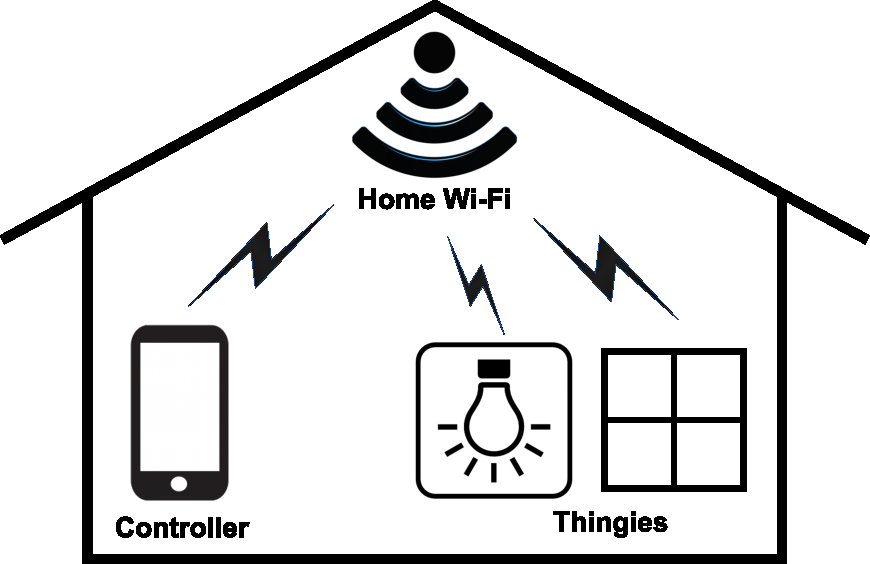
\includegraphics[width=0.90\columnwidth]{figures/systemoverviewdrawing.pdf}
\end{center}
\caption{Overview of the infrastructure}
\label{fig:infrastructureOverview}
\end{figure}

An existing Wi-Fi network in the home provides the communications channel. The user's smartphone is connected to this network. A number of thingies -- exemplified in the figure as a light switch and a window sensor -- are brought into the home and connected to the Wi-Fi network as well. An app on the smartphone then enables the user to control and check on the thingies.

In the rest of this section we will describe each of the critical elements in our proposed infrastructure and discuss our design decisions.

\subsection{Networking, protocols, and Security}

With so many networking technologies available, care must be taken before picking one above another, however, we arrived at our choice, Wi-Fi, pretty fast. One of our primary requirements was that the network should exist in most homes already. This eliminates quite a few choices right away, leaving us with power lines, cellular networks such as 3G, phone line wiring, Bluetooth, and Wi-Fi. Power lines, which have the advantage of reaches all rooms in a home, have problems with the an uncertain network boundaries, since there is usually no special gateway or firewall preventing data from traveling to the neighbours power lines, unless extra hardware is added. Power lines are also inherently a wired network, which means an extra bridge device is needed between the power lines and wireless mobile devices if those are to interact with devices connected to it. The phone lines inside the home have similar problems, and are also far less ubiquitous in the home, with most homes only having a few phone plugs. Then there is Bluetooth, which most laptops and phones, even feature phones, come equipped with. Bluetooth is however limited in range. This leaves cellular networks, which are indeed wireless, but also owned and maintained by carrier companies, that charge fees for the data that travels on their network and not all areas are covered equally well. This makes cellular networks a less ideal choice, landing us squarely on Wi-Fi as the preferred option.

There are many advantages to choosing the Wi-Fi as the basis for our infrastructure and a few drawbacks. Users get to reuse their existing Wi-Fi in their home, thus saving money and time setting up a new device. Wi-Fi also adds, assuming it is protected with a passphrase, a virtual boundary to the smart home, a boundary that users understand because they understand that you cannot access the Wi-Fi without the passphrase. Wi-Fi also have the advantage of being a high bandwidth network which enables thingies such as high resolution CCTV cameras.

The biggest drawback related to Wi-Fi is that it is power hungry compared to other technologies such as ZigBee \cite{zigbeeWebsite}. However, there is a general focus from the Wi-Fi radio chip makers to lower power consumption due to the massive surge of battery driven mobile devices the last few years, so the drawback will matter less as Wi-Fi radios become more power friendly. In addition, for many of the scenarios we have found users to be interested in, thingies will have a permanent power source and in the case where low powered sensor thingies are required, we expect these to use a protocol like ZigBee \cite{zigbeeWebsite} and be bundled with a special purpose thingy which act as a bridge between the individual ZigBee enabled thingies the Wi-Fi network. The bridge thingy could also perform other tasks so the extra cost would be negligible.

We also discussed the problems with oversaturation and general instabilities of the average home Wi-Fi network. This is of course very dependent on the model of the wireless access point used. Better models with good Wi-Fi radios and antennas, faster CPUs, and enough memory, can handle around 25 concurrent connected clients, while lesser models choke at at half as many connections. However, since one of our design goals was that it should be as inexpensive as possible to get started with smart home technology, we do not expect a average home Wi-Fi to get saturated right away. The scenario where a homeowner invests in over 20 new thingies at the same time might not be unlikely, but in that case we feel that investment in an extra access point to handle traffic from thingies is probably also within the budget. Some Wi-Fi experts claim that Wi-Fi clients also have a tendency to drop their connection from access points more often if using the higher bandwidth 802.11n and 802.11g protocols compared to the slower 802.11b. The solution here is to make thingies use 802.11b where possible, and since only a very small subset of thingies will require a 100\% stable connection, homeowners should experience no problems since thingies can simply reconnect if their connection drops.
\subsubsection{Communication protocols}

For communication, we use standard HTTP \cite{Fielding:1999:HTP:RFC2616}. This opens up for a huge list of possible controllers, basically any type of computing device or library that supports HTTP. This is especially important to us since we do not want to be limited to a certain framework, language, or platform, e.g. Java\footnote{\url{http://java.com}} or Android\footnote{\url{http://android.com}}. Other great properties of HTTP is that it is fairly lightweight and stateless protocol \cite{Fielding:1999:HTP:RFC2616}, which simplifies things considerably on the thingies. HTTP also supports our goal of an open infrastructure; it might very well be the best supported protocol among developers, and this enables the average app developer to build new functionality on top of the infrastructure on their platform of choice. Another benefit is that HTTP communication is very unlikely to be blocked by firewalls compared to other less used protocols, so there is a much bigger chance that things will just work.

However, HTTP's statelessness is also a weakness in common smart home scenarios, where a context change in a thingy should trigger an event on a controller. With basic HTTP, a controller waiting for a state change has to continuously poll the thingy it is monitoring to discover the state change in a timely manner. This is an waste of resources and could potentially deplete the resources of a thingy entirely, especially if more controllers are waiting for changes. Clearly, relying only on HTTP alone does not scale. Several solutions to this problem were considered, the biggest contender to be considered being multicast. The advantages of using multicast is that thingies can simply announce state changes on the network and it would not matter how many controllers were interested, the amount of resources required to do so would be the same. Ignoring the problems associated multicast on Wi-Fi, i.e. lost multicast packets are not retransmitted at the MAC layer \cite{conf/icnp/ChandraKMNPRR09}, the reason we did not choose multicast was that the protocol works on a lower level compared to HTTP, and that would limit the number of supported development platforms. We wanted to stay in the Web-stack of technologies so we chose the WebSocket protocol. In the recent years, the WebSocket protocol has been standardized by the Internet Engineering Task Force (IETF) \cite{IETFWebsockets} and is in the process of being standardized by the World Wide Web Consortium (W3C) \cite{w3cWebsockets}. The WebSocket protocol supports multiplexing bi-directional, full-duplex communications channels over a single TCP connection and is already supported by the latests versions of most major browsers\footnote{The WebSocket protocol is supported from Chrome 16, Firefox 11 and Internet Explorer 10.}, with numerous frameworks and libraries already built and more on the way. The WebSocket protocol was essentially designed to be a solution for the scenario where a server needs to push information to a client\cite{IETFWebsockets} which web developers have been struggling with for many years, so while it might not scale as well as multicast, we feel this is the best overall approach.

\subsubsection{Service Discovery}
Most home networks do not have traditional unicast DNS server set up, so we need a different way to discover thingies connect to the network, both during installation and also if and when their IP address changes. We have decided to use mDNS/Bonjour\footnote{Bonjour is available on \url{https://developer.apple.com/opensource/}} since it offers wide support across platforms and is relatively lightweight and open source.
\subsubsection{Security considerations}

The basic trust model for Thingies for Dummies is based on the security of the home's Wi-Fi. Assuming the Wi-Fi is probably configured using WPA2 with AES encryption and a reasonable passphrase, there is a clear boundary for the smart home, and an adversary would not be able to pick up data sent to and from thingies without being connected to the network. This also means, that anyone on the network has full control of the thingies attached to it, which can be a problem in some cases. We have discussed the possibility of adding an extra layer of security that would handle such a case. If the concern is only that unauthorised users cannot perform certain actions on a thingy, i.e. only change state, not update configuration, then we need a way to authenticate each user. This could be done using certificates that clients use to authenticate with. The certificate would be generated during the initial configuration of a thingy, and depending on the number of authorisation levels needed for a thingy, e.g. read only, update state, and update configuration, one or more unique certificates would be generated. Then it would be up to the controller devices used during the initial configuration to distribute the generated certificates to authorized users. However, it is not enough only to authenticate users, since the communication between users and thingies are still being transmitted over an open channel which can allow an adversary to perform replay attacks. The solution to this is to secure the communication channel between users and thinges, i.e. using HTTPS. Adding the extra level of security does raise the hardware requirements on thingies which increases cost and power consumption, so an environment that supports both ``open'', low risk thingies and ``secure'' thingies should provide the best of both worlds.

\subsection{Thingies - actuators and sensors}

To help us narrow down the responsibilities, requirements, and goals for thingies we looked closely at both the scenario described in the introduction of this paper and Edwards et al's \cite{Edwards01athome} work. In summary, thingies should be:

\begin{itemize}
\item Easy to install, maintain, and understand
\item Independent
\item Have a consistent and predictable software interface
\end{itemize}

The first two points are important because thingies must be installable and manageable by less tech-savvy users. It is also reasonable to assume that a simple thingy with one or two functions is going to be more reliable than a device with several functions. Not allowing thingies to be dependent on other thingies or services simplifies everything, which again helps makes things easier for the less tech-savvy user. Making things simple also means being less dependent on constant firmware updates, which will reduce the amount of maintenance required after the initial installation. This is highly important, as Kindberg et al writes, \textit{ ``You can't reboot the world, let alone rewrite it, to introduce new functionality. Users shouldn't be led into a disposable physical world just because they can't keep up with software upgrades.''} \cite{kindbergSystem}.

Thingies can have running logic inside them, depending on their functionality, e.g. a power plug could be configured to turn on and off at specific times during the day, or turn on a secondary output if a specified amount of power is being drawn from a primary output, but it cannot depend on context outside of its domain, i.e. other thingies. Such logic should exist on controllers. Looking back at figure \ref{fig:infrastructureOverview}, recall that the controller is the users's smartphone.

The last point, have a consistent and predictable software interface, is important since controllers and thingies are loosely coupled to each other. A controller must be able to build the visual interface to a thingy without any prior knowledge of it, no matter if the thingy is just a ``read only'' sensor, an actuator or a thingy acting as a bridge for other thingies. To do so, a predictable software interface, in our case, an HTTP-based web service interface is required.

How simple can a thingy be and still be useful? That is a question raised in \cite{Edwards01athome} and it turns out, at least from our informal questioning of friends, family, and colleagues, that even a simple thingy that enables remote toggle of a light switch is useful, and that it is better to have many simple things that end-users are able to comprehend individually instead of one big complex thingy.

\subsubsection{Requirements}

In keeping with the simple theme, we also have very few explicit physical requirements to thingies. They should:

\begin{itemize}
\item Have a unique identifier
\item Have a passive NFC tag and/or a QR code with credentials for its bootstrap access point
\item Have a physical reset/install mode button
\item Be able to connect to an IP based network through a Wi-Fi radio
\end{itemize}

The unique identifier could easily be the MAC address of the Wi-Fi radio or a generic UUID \cite{Leach2005}. A unique ID is required since controllers need a way to identify individual thingies independent of how they are named.

The passive NFC tag or QR code and the physical button are all related to the bootstrapping phase, which we will describe later in this section.

The requirement for a Wi-Fi radio can be weakened to enable the scenario where a ZigBee enabled sensor thingies connect through a specialized ZigBee to Wi-Fi bridge thingy. We do however still require that all thingies can be reached on their own unique URI through the network. This is trivial for thingies connecting directly through Wi-Fi to the home network -- they simply have a standard URI \cite{uri-rfc} based on their IP address, e.g. \texttt{http://192.168.0.42}. In the bridge scenario, the bridged thingies, e.g. ZigBee sensors, may have to share the IP of the bridge. Luckily, the URI schema allows for ports to be defined, so each bridged thingy will be identified by the bridges IP and their own port, e.g. \lstinline{http://192.168.0.42:1337},\\\lstinline{http://192.168.0.42:1338}, etc.

\subsubsection{Web service interface}

Each thingy will have a very basic web service interface consisting of a getter and a setter method, and a method to subscribe to be notified of state changes using the WebSockets protocol. Since controllers have no prior knowledge of thingies, thingies also have a dedicated method which returns a structured description of the their abilities. This makes it possible for the controller to render a UI that lets the user see and manage the state of the thingy.

The structured description associates each state variable in the thingy with ID that is unique within each thingy. This makes it possible update the UI by filling in new state values without reloading the UI description. These IDs are also used when setting the state of the thingy. The following list summarizes the web service interface:

\begin{itemize}
\item \lstinline{/get?id=[list of ids]}\\
Returns the current internal values in the thingy, possibly filtered by ids.
\item \lstinline{/set?id=<id>&value=<value>}\\
Sets the state of a specified internal value in the thingy.
\item \lstinline{/ui}\\
Returns the UI description for the thingy.
\item \lstinline{/subscribe=[list of ids]}\\
Subscribe to live updates of state changes, possibly filtered by ids.
\end{itemize}

The data sent to and from thingies are represented as JSON\footnote{\url{http://json.org/}}. We chose JSON since it is more lightweight than XML, but still structured. It is also easy to parse with libraries available for practically all platforms and languages, and it is aligned with our choice to stick with common web technologies when possible.

\subsubsection{JSON UI Definition Language (JUIDL)}

Inspired by similar work done in the LockIt paper \cite{lockit}, we also defined a JSON based UI definition language, tailored to our needs. The goal for our definition language was that it should convey to controllers \emph{what} type of state is available to controllers, but not \emph{how} that state should be represented visually. This is a similar to XML based Web Service Definition Language (WSDL) \cite{Christensen2001}, however, our JUIDL is much more lightweight, especially since we do not support complex objects.

\subsection{Bootstrapping and installation}

Installing new hardware on a home network is far from trivial, especially when that hardware has little or no UI, and few physical buttons to handle configuration. It is a topic being actively researched in the industry, including the Wi-Fi Alliance\footnote{\url{https://www.wi-fi.org}}. Their 2007 attempt, Wi-Fi Protected Setup (WPS)\footnote{WPS specifications available for purchase at \url{http://www.wi-fi.org/knowledge-center/articles/wi-fi-protected-setup}\texttrademark} was very promising and would have been our choice for easy bootstrapping, but considering the security problems discovered in 2011 \cite{StefanWPS}, we do not feel comfortable depending on a technology that makes Wi-Fi networks insecure if enabled. Instead, we have devised our own bootstrapping protocol.

\subsubsection{Bootstrapping protocol}

Thingies have two modes of operations -- installation mode and normal mode. A thingy can be put in installation mode by pressing a button, and should also arrive in installation mode from the manufacturer. In installation mode, the Wi-Fi radio of the thingy is put in access point mode, allowing another device to connect directly to it to configure it.

The general bootstrapping process is intended to very simple from a user's point of view. First, the user plugs in and turns on the thingy. Then, the user starts the Home Remote app on his smartphone. When the app first runs, it will prompt the user for credentials to the home Wi-Fi network. We considered picking the current network automatically, but we want to ensure that thingies are connected to the right network, and the passphrase is not programmatically retrievable on Android\footnote{\url{http://developer.android.com/reference/android/net/wifi/WifiConfiguration.html}}. Then, the user selects ``Install new thingy''. The onscreen instructions will prompt the user to scan the QR code or hold the phone close to the thingy (if the phone is NFC enabled). From this point, the phone and the thingy are connected to each other, and the user is asked to give the new thingy a name so it is identifiable by humans. The phone also sends the Wi-Fi credentials to the thingy. The diagram in figure \ref{fig:installworkflow} illustrates the workflow of the bootstrapping protocol from a technical point of view.

\begin{figure}[th]
\begin{center}
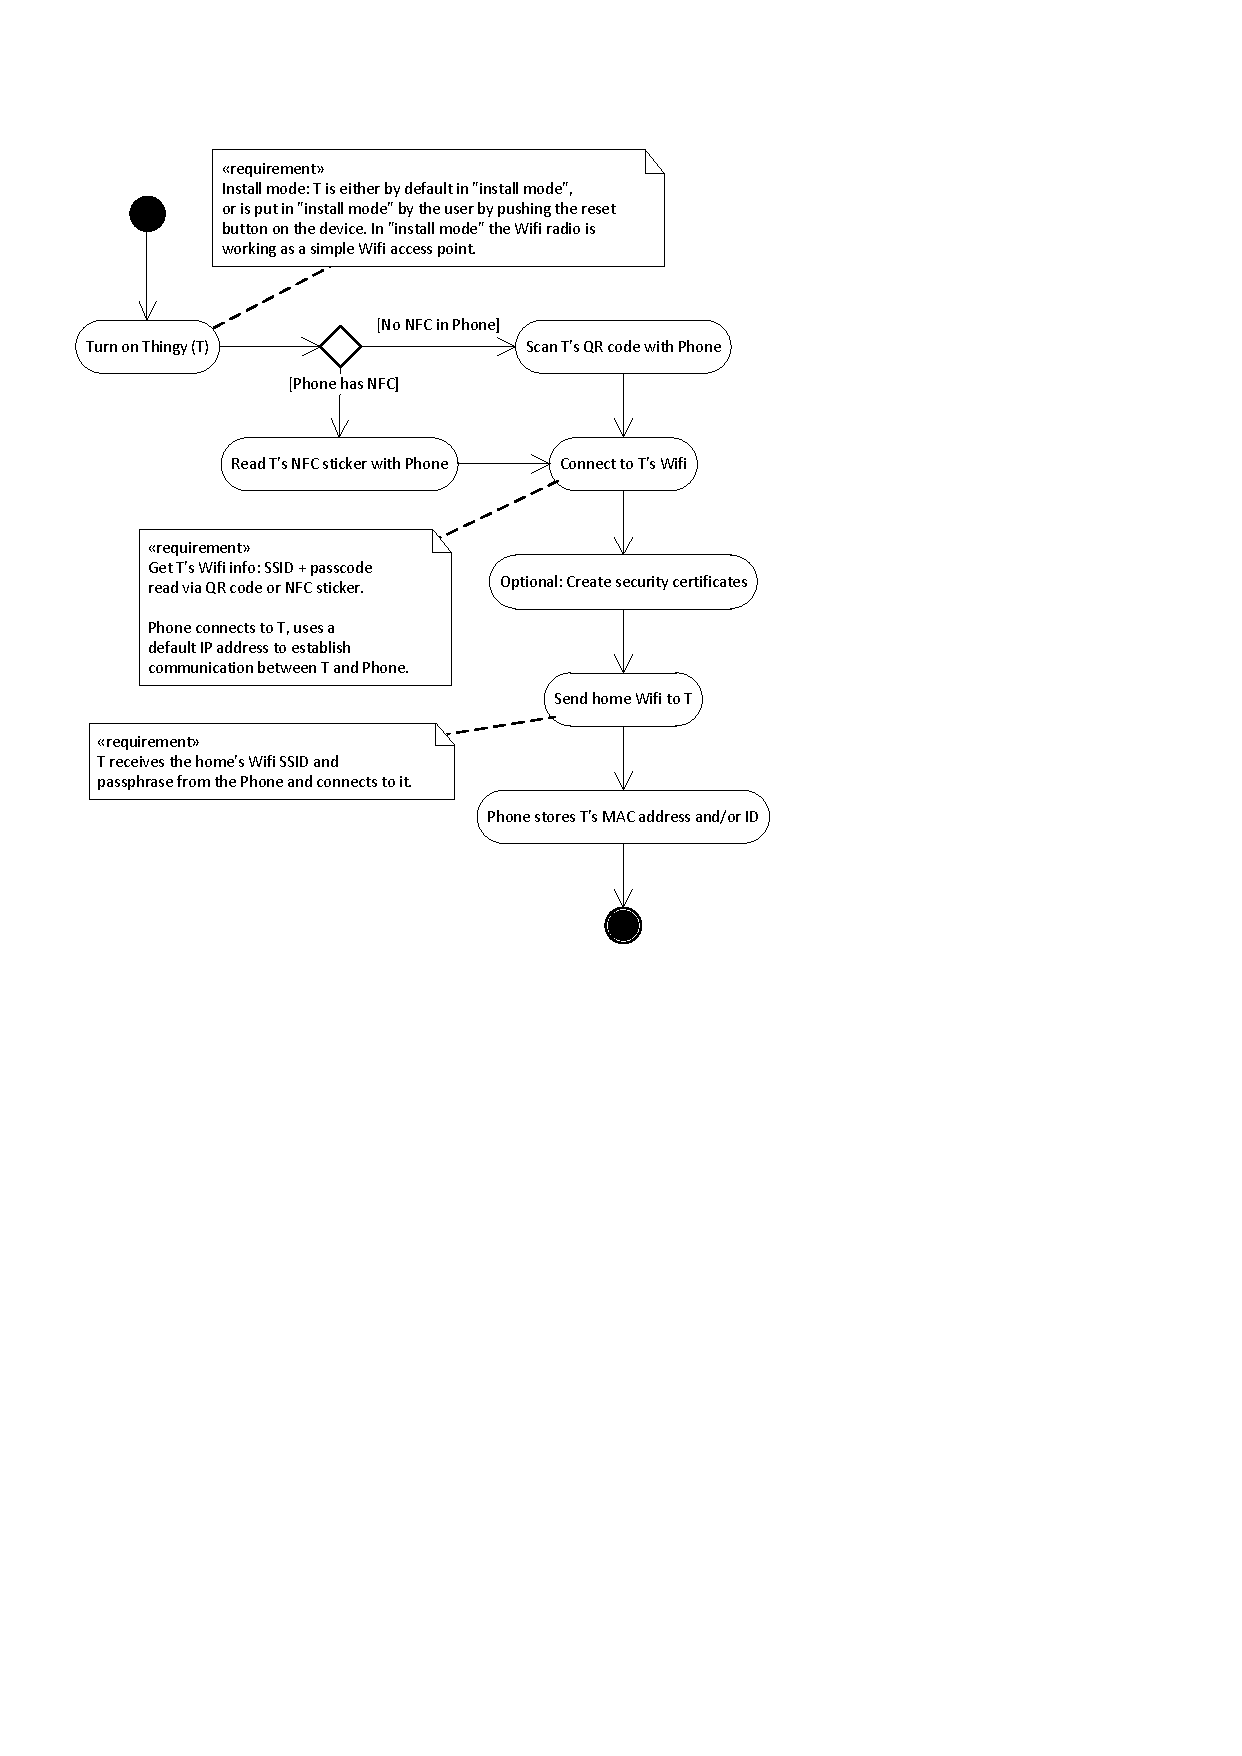
\includegraphics[width=0.90\columnwidth]{figures/installation-workflow.pdf}
\end{center}
\caption{Workflow of the bootstrapping protocol.}
\label{fig:installworkflow}
\end{figure}

Once the thingy is bootstrapped on to the home network, the thingy can be configured regularly through its configuration screen in the Home Remote app.

As for security during bootstrapping, we do not think there is a likely attack vector. When a thingy is in installation mode and has its Wi-Fi radio in access point mode, it will have a passphrase set. With the passphrase randomized, it is very hard for an attacker to get access to a thingy and bootstrap it before the user is able to. Even if this unlikely scenario should occur, the user still retains full physical control over the device, and is able to turn it off or restart the installation process again.

\subsection{Controllers}

You cannot have a smart home without controllers, and to us, the obvious first choice for controllers are smartphones. It is a device which many users carry all the time and are comfortable using. As the previous sections show, we are by no means limited to smartphones -- any computing device supporting the HTTP protocol can act as a controller. This is also our only requirements for simple controllers, although we do require a full controller to be able to perform bootstrapping of new thingies, which is where smartphones really shine.

\subsubsection{End-user programming: Presets}
To enable the simplest form of user programming and automation on the controller level, and to make the scenario described in the introduction possible, we need a way to execute a batch of commands to different thingies. Our solution to this is something we have dubbed ``Presets''. A Preset consists of a name and a set of thingies, along with a desired state for each thingy. When the user defines a new Preset, he gives it a name and then adds one thingy at a time to the preset, specifying which state it should be in.When a Preset is triggered by the user, all thingies in the preset are put in the required state in sequential order, and the expected state of each thingies is checked. If any thingies in the Preset did not end up in the expected state, the user is notified. This also applies to thingies that are only sensors, where the Preset is simply used to verify their states. This enables relatively advanced scenarios such as our ``Lock Down'' scenario described earlier.

This is clearly just the tip of the iceberg in terms of automation. It is easy to imaging additional functionality and in some cases it is simply a matter of enhancing the Preset concept, e.g. having Presets triggered at certain times. When designing more complex automation, there are other issues to consider; e.g. active monitoring of sensors might drain the battery of the phone too fast.

\section{Related Work}

The Internet of Things, implemented in e.g. HP's Cooltown project \cite{cooltown} is a concept related to ours in that it connects the physical and virtual worlds by creating an online presence for physical objects. The Cooltown project also mentions the use of local wireless networks as a means of access restriction.

In the following sections, we will relate our work to other smart home infrastructures as well as other technologies that move user interfaces between devices.

\subsection{Smart home technologies}
Our investigation of smart home technologies has not been as deep as we would have liked -- in part due to time constraints, but also because we did not have access to the relevant equipment. Nevertheless, a comparison follows.

X10\footnote{\url{http://x10.com}, \url{http://www.smarthome.com/about_x10.html}, and \url{http://kbase.x10.com/wiki/MyHouse_Online_Remote_Connection_Setup}} is a low-level protocol from the 70s running through the power lines in a home. It allows one to control a number of devices using a pre-defined set of commands\footnote{url{http://software.x10.com/pub/manuals/xtdcode.pdf}}. Thus, it requires a controller device which is connected to the power lines. When it comes to simplicity and end-user installation, X10 is probably the approach most similar to ours. However, there is the caveat that X10 signals can enter and leave a home through the power lines, so for a secure installation, an electrician is required to install a filtering device. Additionally, X10 does not have the convenience of wireless control built in; this requires the addition of a controller device that supports this.

The Open Services Gateway Initiative, OSGi \cite{osgiIntroduction}, is an infrastructure designed by an alliance of over 80 companies. In \cite{osgiDiscovery}, Dobrev et al. describes how the technology can be used in the context of a smart home, including integration with devices through other technologies such as UPnP and Jini. The approach makes use of a gateway device within the home network. The infrastructure is marketed towards vendors and used in a large number of products and solutions \cite{osgiMarkets}. OSGi is a complex beast, and we have not been able to find an OSGi solution that matches ours in terms of simplicity -- however, we have not investigated all of them.

\subsection{User interface generation}

Since we are designing interaction with UI-less devices -- the thingies -- we will now position our approach in relation to other techniques to move user interfaces from one device to another.

\cite{kindbergSystem} defines four levels of intelligence when moving user interfaces across devices, ranging from e.g. VNC \cite{vnc} where raw pixels and input events are transferred, to e.g. Jini \cite{jini} where the Java code that generates the UI is transferred. In-between, there are approaches where individual widgets are transferred, either by specifying precise widgets (i.e. ``this is a drop down''), or on a purely semantic level (i.e. ``this control must allow selection among these values''). We position ourselves in line with the latter, semantic approach.

\cite{mobileServiceUsage} describes an approach for defining defining mobile user interfaces for web services, by adding two layers on top of the web service definition: one containing a semantic description of the service, and one containing a semantic description of the UI. While this approach may be more generally applicable than ours, it also introduces a considerable complexities.
\section{Implementation}

Due to time constraints, our implementation is limited to a prioritized subset of our designed infrastructure. The implementation includes a sample thingy in the form of a light switch, and a controller in the form of an Android app. We have implemented bootstrapping of the thingy as well as communication between the controller and the thingy.

We have not implemented secure thingies with user authentication, nor is the Android-side of the UI generation implemented beyond what is needed for the sample thingy. The sample thingy requires no configuration, so this has been left out. Also, we opted to use HTTP polling rather than the WebSockets protocol for communication with the thingy. Finally, the bootstrapping process was implemented differently; more on that later.

Our implementation is described in the following. The source code is available online\footnote{\url{https://github.com/egil/dex1}}.

\subsection{Controller: Home Remote for Android}

We implemented a controller as an Android app, dubbed Home Remote. Its initial view (see figure \ref{fig:homeRemoteHomeView}) shows a list of installed thingies along with an option to install new ones. Selecting a thingy shows the user interface for that thingy (same figure).

\begin{figure}[th]
\begin{center}
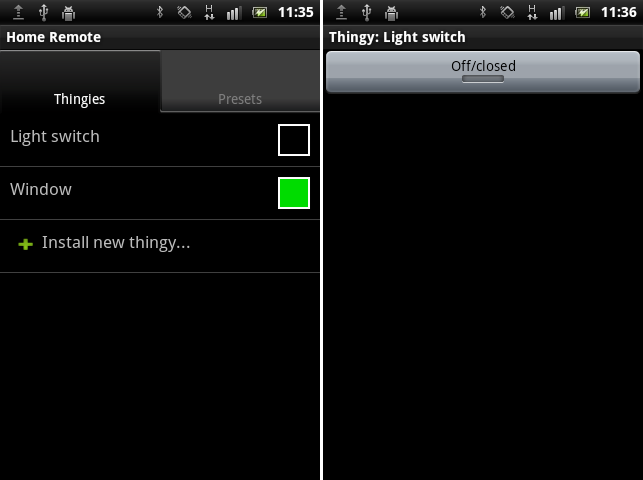
\includegraphics[width=0.90\columnwidth]{figures/home-remote-thingies+1.png}
\end{center}
\caption{Left: The initial view in our controller app. The status of each thingy is shown in a square. Right: The interface for one thingy.}
\label{fig:homeRemoteHomeView}
\end{figure}

\subsubsection{Presets}

Presets have been implemented as described under the heading ``End-user programming: Presets''. A preset consists of a list of thingies along with a desired status for each thingy (figure \ref{fig:homeRemotePresets}). Activating a preset causes thingies with actuators to change state, while thingies with sensors are listed to let the preset function as a check list. Check marks are overlaid on the status icons of thingies to indicate whether each thingy is in the desired state (see figure \ref{fig:homeRemotePresets}).

\begin{figure}[th]
\begin{center}
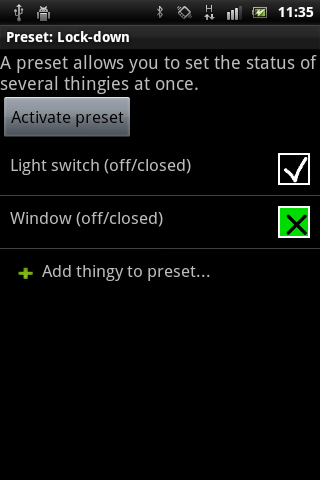
\includegraphics[width=0.45\columnwidth]{figures/home-remote-preset.png}
\end{center}
\caption{A preset in our controller app. The light is off as desired, but the window is still open.}
\label{fig:homeRemotePresets}
\end{figure}

\subsection{Thingy: Light switch}

Our sample thingy, a light switch, was implemented on an Arduino board, with a WiFly shield\footnote{\url{http://www.sparkfun.com/products/9954}} for Wi-Fi connectivity. A relay was used in a circuit based on an example at the Arduino website\footnote{\url{http://www.arduino.cc/playground/uploads/Learning/relays.pdf}}, except with a 480$\Omega$ resistor and two transistors mounted as a Darlington pair\footnote{\url{http://en.wikipedia.org/wiki/Darlington_transistor}}. Once installed, this thingy allows one to control a power outlet and thus, for instance, a lamp.
\subsection{The bootstrap process}

Recall that the purpose of our bootstrap process is to get a new thingy connected to the home Wi-Fi. In the design, we had envisioned a bootstrap process where the thingy would provide a temporary access point that the Android app could connect to for initial communication. However, it turned out that while the WiFly board supports ad hoc mode, it cannot work as a regular access point\footnote{\url{http://www.sparkfun.com/datasheets/Wireless/WiFi/WiFlyGSX-um2.pdf}}. Ad hoc mode is, in turn, not supported by Android phones out of the box\footnote{\url{http://szym.net/2010/12/adhoc-wifi-in-android/}}. However, since Android phones \emph{are} able to work as regular access points, we decided to turn the process around:

\begin{figure}[th]
\begin{center}
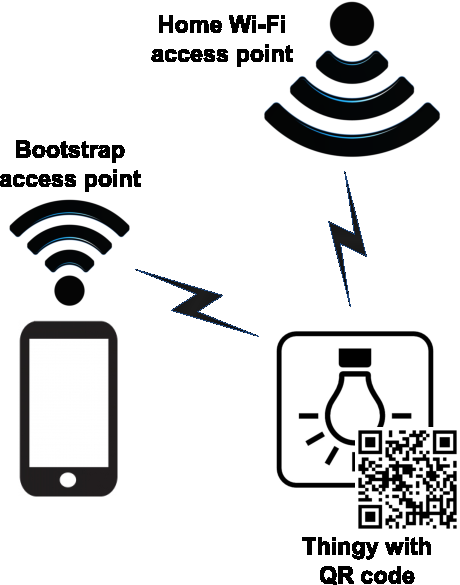
\includegraphics[width=0.70\columnwidth]{figures/bootstrap-drawing.pdf}
\end{center}
\caption{Devices and access points involved in the bootstrap process}
\label{fig:bootstrapDraw}
\end{figure}

When the user starts the process by selecting ``Install new thingy'' in the Android app, the user is first prompted to scan the QR code that came with the thingy. This code contains the SSID and passphrase of the bootstrap access point that the app then sets up on the phone. Second, the app instructs the user to press the button on the thingy; this causes the thingy to make a request to the Android phone via the bootstrap access point. The response to this request contains the SSID and passphrase of the home Wi-Fi access point, which the thingy then connects to, obtaining an IP address. Next, the thingy briefly reconnects to the bootstrap access point to send this IP address to the Android app. Finally, the thingy reconnects to the home Wi-Fi, and the Android app closes the bootstrap access point and reconnects to the home Wi-Fi as well. Thus, the thingy is connected to the home Wi-Fi and the Android app is able to make requests to the thingy.

One disadvantage of this implementation is the use of an undocumented API call\footnote{\url{http://stackoverflow.com/questions/3023226/android-2-2-wifi-hotspot-api}}, another is the fact that older Android phones cannot work as access points, and third it relies on the home access point issuing the same IP address when the thingy reconnects. For these reasons, we would still recommend an implementation closer to our design. That being said, our implementation works, and the user experience is the same as we had envisioned.
\section{Evaluation}

The evaluation of our concept and prototype was performed in three phases: first, an initial evaluation of the overall idea, second, an evaluation of an early prototype using the ``Wizard of Oz'' technique \cite{wizardOfOz}, and third, an evaluation of the final prototype. Each is described in the following.
\subsection{Initial evaluation of the idea}

Before setting out to develop a prototype, we wanted to be sure that our idea was useful. Therefore, we checked with a number of friends and colleagues. We used short, semi-structured interviews, asking ``Would you be interested in controlling something in your home from your phone, and if so, what would it be?''. We also told them that controlling objects while away from home was a possibility. Nine or ten participants were asked.

We generally received a moderate amount of interest -- it was not the case that everyone was instantly thrilled by the possibility, but all participants did think of something that they would actually like to remote control, either from inside or outside the home. The ideas are listed in the introduction.

This assured us that it was worthwhile to proceed.
\subsection{Evaluation of the first prototype}

In order to evaluate a prototype as early as possible, we decided to use a ``Wizard of Oz''-approach where we faked the parts of the system that were the least perceptible for the participants. We thus implemented the interface for the Home Remote Android app that the participants would interact with directly. A fake thingy was built in the form of a light switch -- in reality, a physical switch at the end of an extension cord allowed the ``wizard'' to turn the light on or off according to the participant's interaction with the app. Similarly, the association of the fake thingy with the home Wi-Fi was simulated. A simple web interface, shown in figure \ref{fig:wizardInterface}, let the test conductor see and change the status of thingies that was shown in the app.

\begin{figure}[th]
\begin{center}
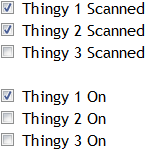
\includegraphics[width=0.4\columnwidth]{figures/prototype-wizard-interface.png}
\end{center}
\caption{Web interface for the wizard. The ``scanned'' boxes indicate whether the thingies are connected to Wi-Fi while the ``on'' boxes indicate their status.}
\label{fig:wizardInterface}
\end{figure}

The evaluation focused on the installation process, the concept of remote control, the concept of presets, and the overall usefulness of our idea. An installation guide\footnote{\url{https://github.com/egil/DEX1/blob/master/report/extras/installation-guide.pdf}} was handed out, and we asked participants to install the thingy, remotely control it, and then to set up and use a preset. This was followed by a semi-structured interview where we asked participants what they liked and didn't like about the system, if there was anything they did not understand, and what they would change. For details on the evaluation procedure and the interview questions, see the evaluation document\footnote{\url{https://github.com/egil/DEX1/blob/master/report/extras/evaluation-plan.pdf}}.

 In order to evaluate the ease of installation, we selected two less tech-savvy, middle-aged participants, one of which already owned a smart phone. While the number of participants for this evaluation was indeed limited due to time constraints, we still believe that the results are useful -- especially where there are similarities in the reactions.

The ``Wizard of Oz''-approach worked surprisingly well as participants forgot about the extension cord and were surprised to see the the light control working. This system introduced a new causal relationship \cite{causalReasoning}, i.e. interacting with the app caused lights to go on and off, and participants quickly picked up on this.

Neither participant found it immediately obvious how to control a thingy from the app after having installed the thingy, so the interface needs some tweaks in this regard. The concept of presets required some explaining, and with only one physical thingy it proved difficult to provide the illusion of controlling several thingies at once.

Both participants were mostly interested in remote scenarios -- e.g. checking that everything was in order after having left the home. This shows us that we do indeed need to cross the boundary of the home Wi-Fi, perhaps through a cloud service or a gateway device in the home.

\subsection{Evaluation of the final prototype}

For the final prototype, we set out to implement a light switch. With the bootstrapping implemented, we were able to to evaluate the installation process. As we were, despite an enthusiastic attempt, unable to build the circuitry to control an actual switch in time for the evaluation, we opted not to evaluate regular use at this point.

We selected two participants in their early twenties. Both had experience with smartphones but were not overwhelmingly tech savvy. Neither participant had been part of the previous evaluation. This time, participants were only asked to install our prototype thingy, i.e. to perform the bootstrapping procedure. This was followed by a semi-structured interview based on the same questions as previously, skipping the ones that did not apply.

\begin{figure}[th]
\begin{center}
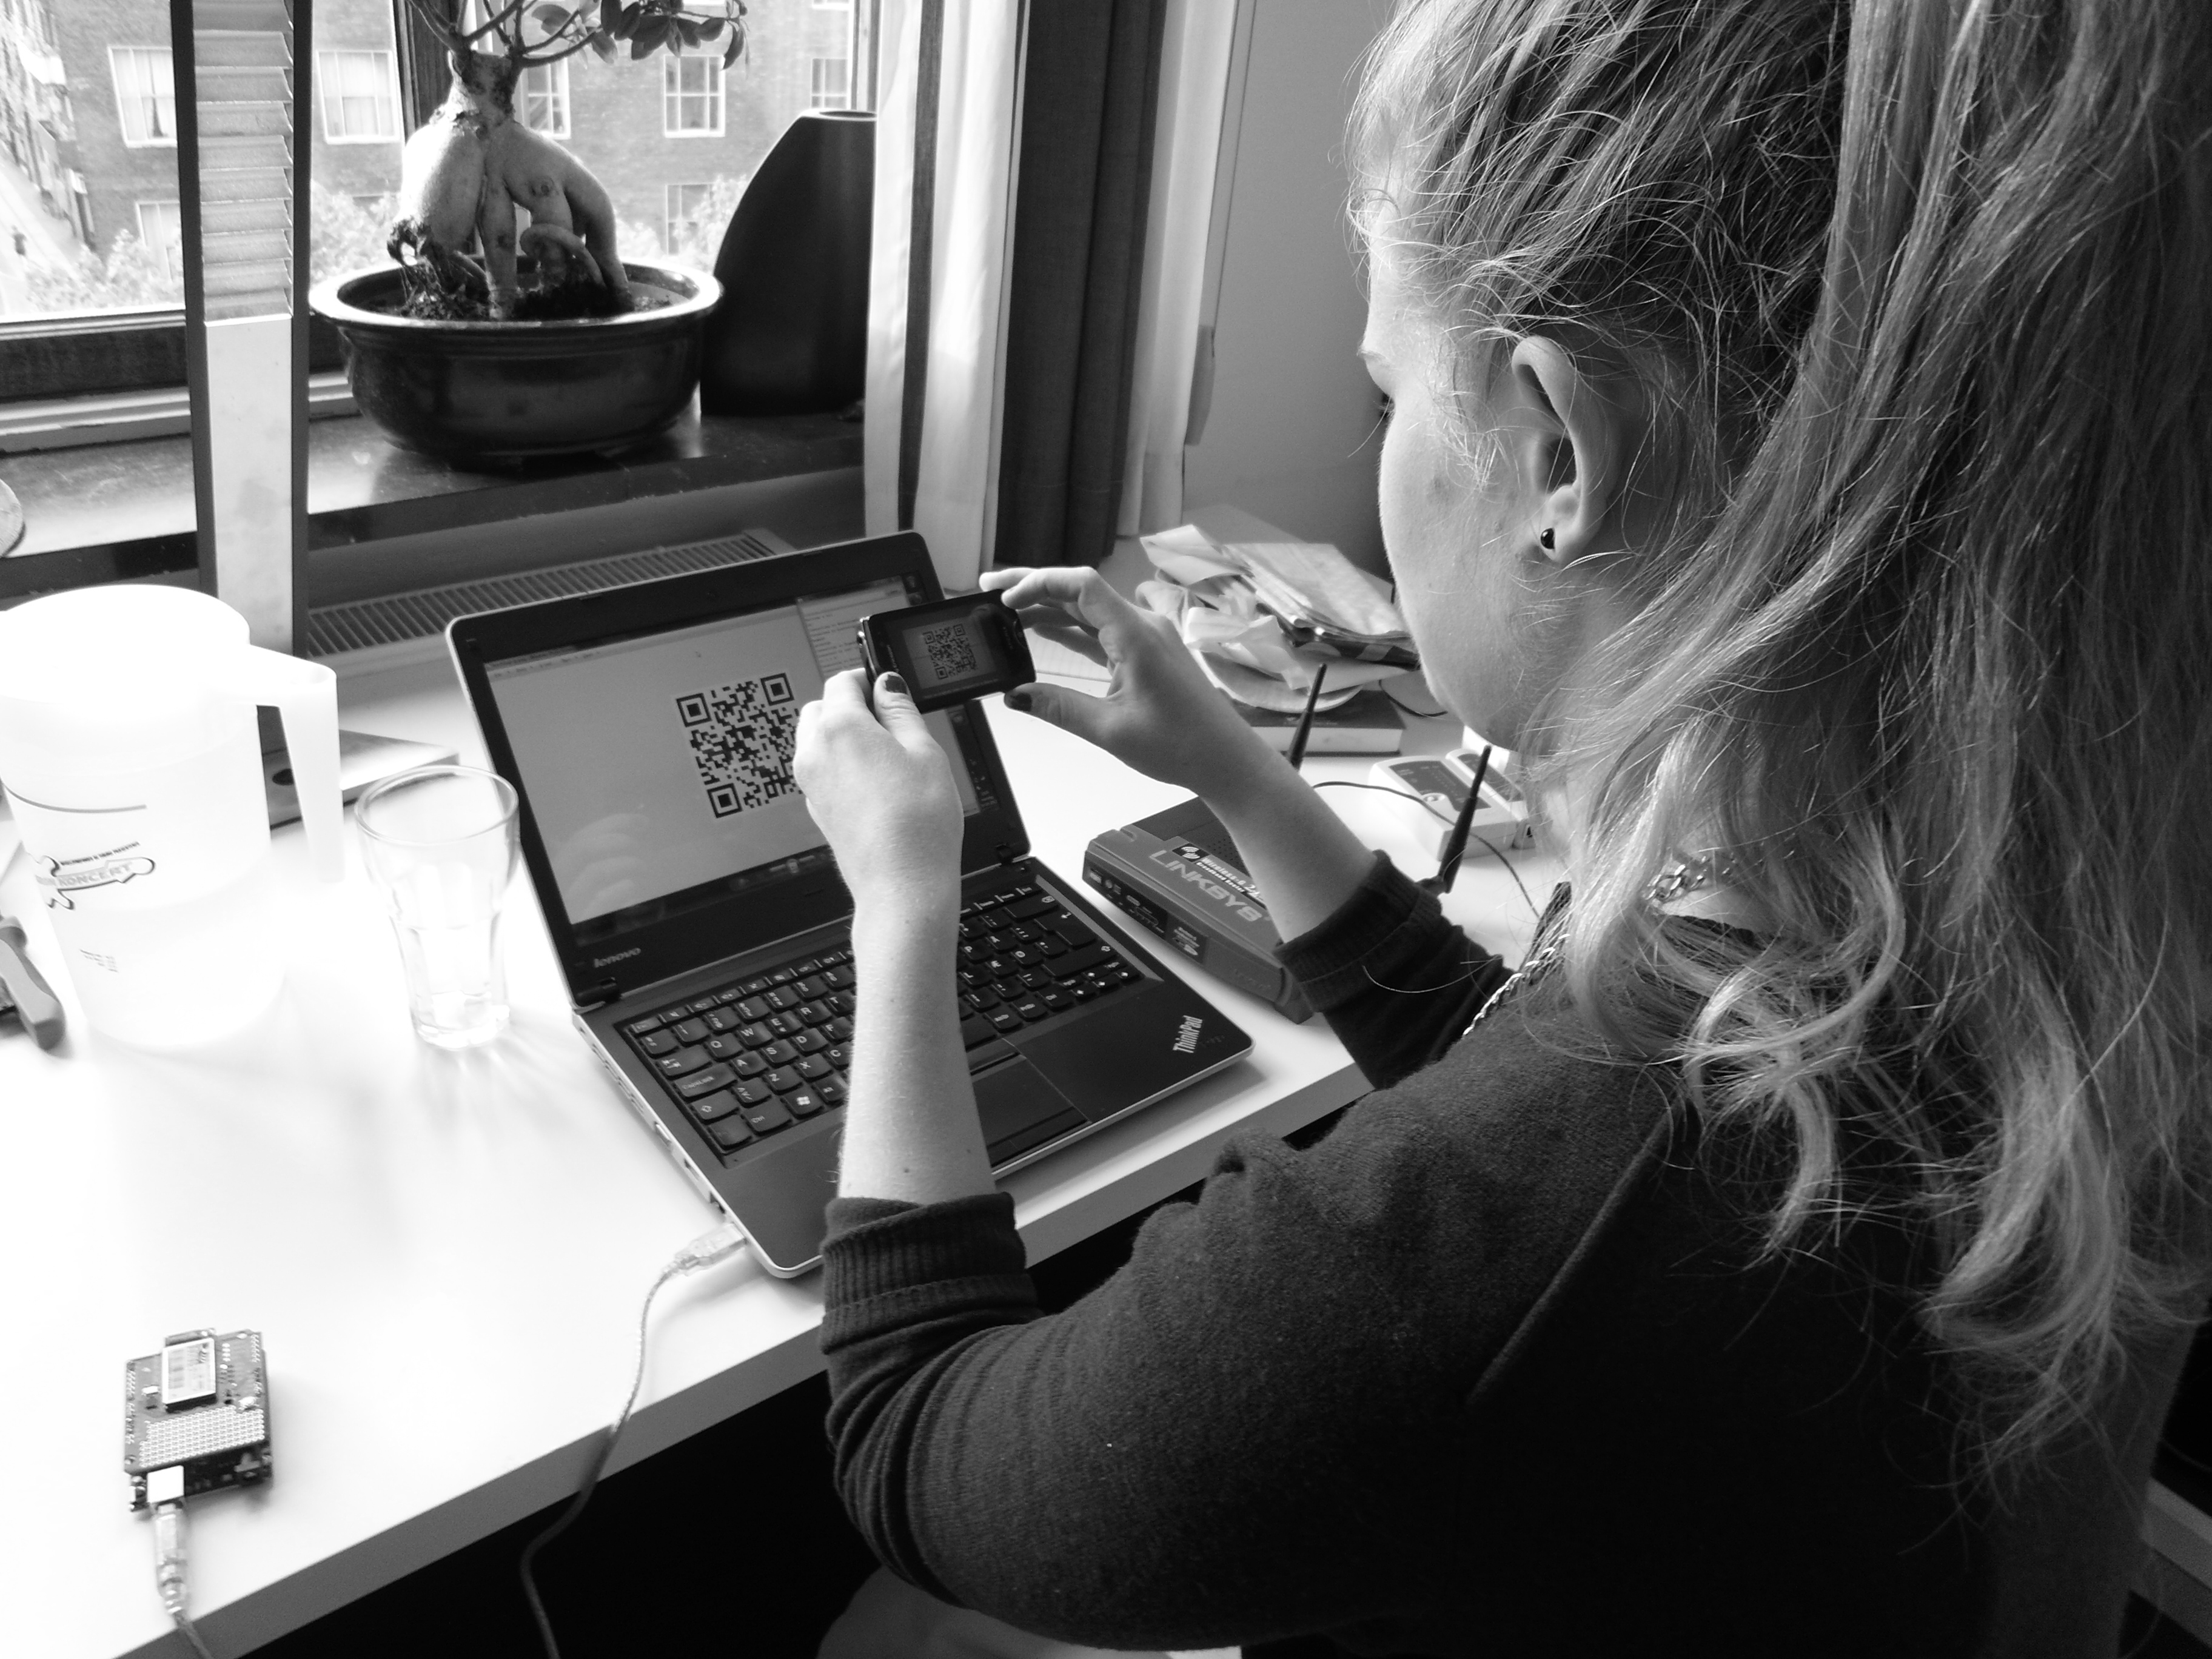
\includegraphics[width=0.90\columnwidth]{figures/evaluation-picture.jpg}
\end{center}
\caption{Evaluation of the bootstrapping process. The participant is scanning the QR code.}
\label{fig:evalPic}
\end{figure}

Both participants found that the process was simple and easy to follow overall, one stating that the process was well-guided by the app. One participant pointed out that there was a lack of feedback during the process -- the bootstrapping took around 20 seconds with a static text indicating that it would take ``a little while''. This was especially apparent when the thingy failed connecting in the first attempt and required an extra button push. The other participant had not previously scanned a QR code and thus found this a little less intuitive than we had anticipated.

\section{Discussion}

Our evaluation indicates that it is indeed possible to make smart home technology accessible to less tech-savvy users, though a more thorough evaluation is needed. There are still questions as to the complexity of physically installing thingies: this cannot be more complicated than it is to assemble furniture from IKEA.

While one might argue that we are missing a complete evaluation of the final prototype, we do feel that we have covered our implementation by evaluating both regular use and the installation process over the course of the project.

It is on the controller that we envision the platform to take shape in a similar way to e.g. the Android platform. We imagine, that the technologies that developers already understand, will enable new innovative ways to control the home. It was clear from our evaluations that users really like the away from home scenarios, and it is probably no coincidence that big companies like AT\&T and IBM are pursuing this through cloud based services. Our proposed infrastructure is in no way in conflict with this cloud based approach, quite the opposite, since all thingies are IP based already. Enabling a cloud scenario with our infrastructure should only require a gateway device that keeps a connection to the cloud service and a connection to each thingy inside the home network.

Multi-user scenarios add interesting issues that we have not looked into in depth: one is the synchronization of configuration between controllers, another is the privacy issues that might arise when users are suddenly able to remotely monitor and affect physical objects in the home. We are more or less used to being actively monitored in some capacity when we leave the home, but will people feel comfortable being monitored while at home?
\section{Conclusion}

In this paper, we have described an infrastructure that allows anyone to retrofit their home with pieces of smart home technology while leveraging existing equipment. We have implemented a subset of our design in a prototype, and through our evaluation we have seen that this prototype is indeed easy to install and use, though a few tweaks to the user interface would improve the user experience. Our infrastructure includes a secure bootstrapping process where UI-less devices are connected to a user's Wi-Fi network.

\section{Acknowledgements}

We would like to thank Jakob Bardram, Sebastian B\"{u}ttrich, and especially Thomas Pederson for excellent supervision. A thank-you is also due for the guys at Brinck's Elektronik\footnote{\url{http://elextra.dk}}, and to those who participated in our evaluation.

\bibliographystyle{abbrv}
\bibliography{bibliography}

\end{document}